\documentclass[]{article}
\usepackage{lmodern}
\usepackage{amssymb,amsmath}
\usepackage{ifxetex,ifluatex}
\usepackage{fixltx2e} % provides \textsubscript
\ifnum 0\ifxetex 1\fi\ifluatex 1\fi=0 % if pdftex
  \usepackage[T1]{fontenc}
  \usepackage[utf8]{inputenc}
\else % if luatex or xelatex
  \ifxetex
    \usepackage{mathspec}
  \else
    \usepackage{fontspec}
  \fi
  \defaultfontfeatures{Ligatures=TeX,Scale=MatchLowercase}
\fi
% use upquote if available, for straight quotes in verbatim environments
\IfFileExists{upquote.sty}{\usepackage{upquote}}{}
% use microtype if available
\IfFileExists{microtype.sty}{%
\usepackage{microtype}
\UseMicrotypeSet[protrusion]{basicmath} % disable protrusion for tt fonts
}{}
\usepackage[margin=2.54cm]{geometry}
\usepackage{hyperref}
\hypersetup{unicode=true,
            pdftitle={Assignment 5: Data Visualization},
            pdfauthor={Lehe Xu},
            pdfborder={0 0 0},
            breaklinks=true}
\urlstyle{same}  % don't use monospace font for urls
\usepackage{color}
\usepackage{fancyvrb}
\newcommand{\VerbBar}{|}
\newcommand{\VERB}{\Verb[commandchars=\\\{\}]}
\DefineVerbatimEnvironment{Highlighting}{Verbatim}{commandchars=\\\{\}}
% Add ',fontsize=\small' for more characters per line
\usepackage{framed}
\definecolor{shadecolor}{RGB}{248,248,248}
\newenvironment{Shaded}{\begin{snugshade}}{\end{snugshade}}
\newcommand{\AlertTok}[1]{\textcolor[rgb]{0.94,0.16,0.16}{#1}}
\newcommand{\AnnotationTok}[1]{\textcolor[rgb]{0.56,0.35,0.01}{\textbf{\textit{#1}}}}
\newcommand{\AttributeTok}[1]{\textcolor[rgb]{0.77,0.63,0.00}{#1}}
\newcommand{\BaseNTok}[1]{\textcolor[rgb]{0.00,0.00,0.81}{#1}}
\newcommand{\BuiltInTok}[1]{#1}
\newcommand{\CharTok}[1]{\textcolor[rgb]{0.31,0.60,0.02}{#1}}
\newcommand{\CommentTok}[1]{\textcolor[rgb]{0.56,0.35,0.01}{\textit{#1}}}
\newcommand{\CommentVarTok}[1]{\textcolor[rgb]{0.56,0.35,0.01}{\textbf{\textit{#1}}}}
\newcommand{\ConstantTok}[1]{\textcolor[rgb]{0.00,0.00,0.00}{#1}}
\newcommand{\ControlFlowTok}[1]{\textcolor[rgb]{0.13,0.29,0.53}{\textbf{#1}}}
\newcommand{\DataTypeTok}[1]{\textcolor[rgb]{0.13,0.29,0.53}{#1}}
\newcommand{\DecValTok}[1]{\textcolor[rgb]{0.00,0.00,0.81}{#1}}
\newcommand{\DocumentationTok}[1]{\textcolor[rgb]{0.56,0.35,0.01}{\textbf{\textit{#1}}}}
\newcommand{\ErrorTok}[1]{\textcolor[rgb]{0.64,0.00,0.00}{\textbf{#1}}}
\newcommand{\ExtensionTok}[1]{#1}
\newcommand{\FloatTok}[1]{\textcolor[rgb]{0.00,0.00,0.81}{#1}}
\newcommand{\FunctionTok}[1]{\textcolor[rgb]{0.00,0.00,0.00}{#1}}
\newcommand{\ImportTok}[1]{#1}
\newcommand{\InformationTok}[1]{\textcolor[rgb]{0.56,0.35,0.01}{\textbf{\textit{#1}}}}
\newcommand{\KeywordTok}[1]{\textcolor[rgb]{0.13,0.29,0.53}{\textbf{#1}}}
\newcommand{\NormalTok}[1]{#1}
\newcommand{\OperatorTok}[1]{\textcolor[rgb]{0.81,0.36,0.00}{\textbf{#1}}}
\newcommand{\OtherTok}[1]{\textcolor[rgb]{0.56,0.35,0.01}{#1}}
\newcommand{\PreprocessorTok}[1]{\textcolor[rgb]{0.56,0.35,0.01}{\textit{#1}}}
\newcommand{\RegionMarkerTok}[1]{#1}
\newcommand{\SpecialCharTok}[1]{\textcolor[rgb]{0.00,0.00,0.00}{#1}}
\newcommand{\SpecialStringTok}[1]{\textcolor[rgb]{0.31,0.60,0.02}{#1}}
\newcommand{\StringTok}[1]{\textcolor[rgb]{0.31,0.60,0.02}{#1}}
\newcommand{\VariableTok}[1]{\textcolor[rgb]{0.00,0.00,0.00}{#1}}
\newcommand{\VerbatimStringTok}[1]{\textcolor[rgb]{0.31,0.60,0.02}{#1}}
\newcommand{\WarningTok}[1]{\textcolor[rgb]{0.56,0.35,0.01}{\textbf{\textit{#1}}}}
\usepackage{graphicx,grffile}
\makeatletter
\def\maxwidth{\ifdim\Gin@nat@width>\linewidth\linewidth\else\Gin@nat@width\fi}
\def\maxheight{\ifdim\Gin@nat@height>\textheight\textheight\else\Gin@nat@height\fi}
\makeatother
% Scale images if necessary, so that they will not overflow the page
% margins by default, and it is still possible to overwrite the defaults
% using explicit options in \includegraphics[width, height, ...]{}
\setkeys{Gin}{width=\maxwidth,height=\maxheight,keepaspectratio}
\IfFileExists{parskip.sty}{%
\usepackage{parskip}
}{% else
\setlength{\parindent}{0pt}
\setlength{\parskip}{6pt plus 2pt minus 1pt}
}
\setlength{\emergencystretch}{3em}  % prevent overfull lines
\providecommand{\tightlist}{%
  \setlength{\itemsep}{0pt}\setlength{\parskip}{0pt}}
\setcounter{secnumdepth}{0}
% Redefines (sub)paragraphs to behave more like sections
\ifx\paragraph\undefined\else
\let\oldparagraph\paragraph
\renewcommand{\paragraph}[1]{\oldparagraph{#1}\mbox{}}
\fi
\ifx\subparagraph\undefined\else
\let\oldsubparagraph\subparagraph
\renewcommand{\subparagraph}[1]{\oldsubparagraph{#1}\mbox{}}
\fi

%%% Use protect on footnotes to avoid problems with footnotes in titles
\let\rmarkdownfootnote\footnote%
\def\footnote{\protect\rmarkdownfootnote}

%%% Change title format to be more compact
\usepackage{titling}

% Create subtitle command for use in maketitle
\providecommand{\subtitle}[1]{
  \posttitle{
    \begin{center}\large#1\end{center}
    }
}

\setlength{\droptitle}{-2em}

  \title{Assignment 5: Data Visualization}
    \pretitle{\vspace{\droptitle}\centering\huge}
  \posttitle{\par}
    \author{Lehe Xu}
    \preauthor{\centering\large\emph}
  \postauthor{\par}
    \date{}
    \predate{}\postdate{}
  

\begin{document}
\maketitle

\hypertarget{overview}{%
\subsection{OVERVIEW}\label{overview}}

This exercise accompanies the lessons in Environmental Data Analytics on
Data Visualization

\hypertarget{directions}{%
\subsection{Directions}\label{directions}}

\begin{enumerate}
\def\labelenumi{\arabic{enumi}.}
\tightlist
\item
  Change ``Student Name'' on line 3 (above) with your name.
\item
  Work through the steps, \textbf{creating code and output} that fulfill
  each instruction.
\item
  Be sure to \textbf{answer the questions} in this assignment document.
\item
  When you have completed the assignment, \textbf{Knit} the text and
  code into a single PDF file.
\item
  After Knitting, submit the completed exercise (PDF file) to the
  dropbox in Sakai. Add your last name into the file name (e.g.,
  ``Fay\_A05\_DataVisualization.Rmd'') prior to submission.
\end{enumerate}

The completed exercise is due on Monday, February 14 at 7:00 pm.

\hypertarget{set-up-your-session}{%
\subsection{Set up your session}\label{set-up-your-session}}

\begin{enumerate}
\def\labelenumi{\arabic{enumi}.}
\tightlist
\item
  Set up your session. Verify your working directory and load the
  tidyverse and cowplot packages. Upload the NTL-LTER processed data
  files for nutrients and chemistry/physics for Peter and Paul Lakes
  (use the tidy
  {[}\texttt{NTL-LTER\_Lake\_Chemistry\_Nutrients\_PeterPaul\_Processed.csv}{]}
  version) and the processed data file for the Niwot Ridge litter
  dataset (use the
  {[}\texttt{NEON\_NIWO\_Litter\_mass\_trap\_Processed.csv}{]} version).
\end{enumerate}

\begin{Shaded}
\begin{Highlighting}[]
\CommentTok{\#1}
\FunctionTok{getwd}\NormalTok{()}
\end{Highlighting}
\end{Shaded}

\begin{verbatim}
## [1] "D:/Documents/Environmental_Data_Analytics_2022"
\end{verbatim}

\begin{Shaded}
\begin{Highlighting}[]
\FunctionTok{library}\NormalTok{(tidyverse)}
\end{Highlighting}
\end{Shaded}

\begin{verbatim}
## Warning: package 'tidyverse' was built under R version 3.6.3
\end{verbatim}

\begin{verbatim}
## -- Attaching packages ---------------------------------- tidyverse 1.3.1 --
\end{verbatim}

\begin{verbatim}
## v ggplot2 3.3.5     v purrr   0.3.4
## v tibble  3.1.1     v dplyr   1.0.6
## v tidyr   1.1.3     v stringr 1.4.0
## v readr   1.4.0     v forcats 0.5.1
\end{verbatim}

\begin{verbatim}
## Warning: package 'tibble' was built under R version 3.6.3
\end{verbatim}

\begin{verbatim}
## Warning: package 'tidyr' was built under R version 3.6.3
\end{verbatim}

\begin{verbatim}
## Warning: package 'readr' was built under R version 3.6.3
\end{verbatim}

\begin{verbatim}
## Warning: package 'purrr' was built under R version 3.6.3
\end{verbatim}

\begin{verbatim}
## Warning: package 'dplyr' was built under R version 3.6.3
\end{verbatim}

\begin{verbatim}
## Warning: package 'forcats' was built under R version 3.6.3
\end{verbatim}

\begin{verbatim}
## -- Conflicts ------------------------------------- tidyverse_conflicts() --
## x dplyr::filter() masks stats::filter()
## x dplyr::lag()    masks stats::lag()
\end{verbatim}

\begin{Shaded}
\begin{Highlighting}[]
\FunctionTok{library}\NormalTok{(ggridges)}
\end{Highlighting}
\end{Shaded}

\begin{verbatim}
## Warning: package 'ggridges' was built under R version 3.6.3
\end{verbatim}

\begin{Shaded}
\begin{Highlighting}[]
\NormalTok{NTL }\OtherTok{\textless{}{-}} 
  \FunctionTok{read.csv}\NormalTok{(}\StringTok{"./Data/Processed/NTL{-}LTER\_Lake\_Chemistry\_Nutrients\_PeterPaul\_Processed.csv"}\NormalTok{, }
           \AttributeTok{stringsAsFactors =} \ConstantTok{TRUE}\NormalTok{)}
\NormalTok{NEON }\OtherTok{\textless{}{-}}
  \FunctionTok{read.csv}\NormalTok{(}\StringTok{"./Data/Processed/NEON\_NIWO\_Litter\_mass\_trap\_Processed.csv"}\NormalTok{, }\AttributeTok{stringsAsFactors =} \ConstantTok{TRUE}\NormalTok{)}
\end{Highlighting}
\end{Shaded}

\begin{enumerate}
\def\labelenumi{\arabic{enumi}.}
\setcounter{enumi}{1}
\tightlist
\item
  Make sure R is reading dates as date format; if not change the format
  to date.
\end{enumerate}

\begin{Shaded}
\begin{Highlighting}[]
\CommentTok{\#2}
\NormalTok{NTL}\SpecialCharTok{$}\NormalTok{sampledate }\OtherTok{\textless{}{-}} \FunctionTok{as.Date}\NormalTok{(NTL}\SpecialCharTok{$}\NormalTok{sampledate, }\AttributeTok{format =} \StringTok{"\%Y{-}\%m{-}\%d"}\NormalTok{)}
\NormalTok{NEON}\SpecialCharTok{$}\NormalTok{collectDate }\OtherTok{\textless{}{-}} \FunctionTok{as.Date}\NormalTok{(NEON}\SpecialCharTok{$}\NormalTok{collectDate, }\AttributeTok{format =} \StringTok{"\%Y{-}\%m{-}\%d"}\NormalTok{)}
\end{Highlighting}
\end{Shaded}

\hypertarget{define-your-theme}{%
\subsection{Define your theme}\label{define-your-theme}}

\begin{enumerate}
\def\labelenumi{\arabic{enumi}.}
\setcounter{enumi}{2}
\tightlist
\item
  Build a theme and set it as your default theme.
\end{enumerate}

\begin{Shaded}
\begin{Highlighting}[]
\CommentTok{\#3}
\NormalTok{mytheme }\OtherTok{\textless{}{-}} \FunctionTok{theme\_classic}\NormalTok{(}\AttributeTok{base\_size =} \DecValTok{14}\NormalTok{) }\SpecialCharTok{+}
  \FunctionTok{theme}\NormalTok{(}\AttributeTok{axis.text =} \FunctionTok{element\_text}\NormalTok{(}\AttributeTok{color =} \StringTok{"darkblue"}\NormalTok{), }
        \AttributeTok{legend.position =} \StringTok{"bottom"}\NormalTok{)}

\FunctionTok{theme\_set}\NormalTok{(mytheme)}
\end{Highlighting}
\end{Shaded}

\hypertarget{create-graphs}{%
\subsection{Create graphs}\label{create-graphs}}

For numbers 4-7, create ggplot graphs and adjust aesthetics to follow
best practices for data visualization. Ensure your theme, color
palettes, axes, and additional aesthetics are edited accordingly.

\begin{enumerate}
\def\labelenumi{\arabic{enumi}.}
\setcounter{enumi}{3}
\tightlist
\item
  {[}NTL-LTER{]} Plot total phosphorus (\texttt{tp\_ug}) by phosphate
  (\texttt{po4}), with separate aesthetics for Peter and Paul lakes. Add
  a line of best fit and color it black. Adjust your axes to hide
  extreme values (hint: change the limits using \texttt{xlim()} and
  \texttt{ylim()}).
\end{enumerate}

\begin{Shaded}
\begin{Highlighting}[]
\CommentTok{\#4}
\NormalTok{tp.po4 }\OtherTok{\textless{}{-}}
  \FunctionTok{ggplot}\NormalTok{(NTL, }\FunctionTok{aes}\NormalTok{(}\AttributeTok{x =}\NormalTok{ po4, }\AttributeTok{y =}\NormalTok{ tp\_ug, }\AttributeTok{color =}\NormalTok{ lakename)) }\SpecialCharTok{+}
  \FunctionTok{geom\_point}\NormalTok{() }\SpecialCharTok{+}
  \FunctionTok{geom\_smooth}\NormalTok{(}\AttributeTok{method =}\NormalTok{ lm, }\AttributeTok{color=}\StringTok{"black"}\NormalTok{)}\SpecialCharTok{+}
  \FunctionTok{xlim}\NormalTok{(}\DecValTok{0}\NormalTok{, }\DecValTok{50}\NormalTok{) }
  \FunctionTok{ylim}\NormalTok{(}\DecValTok{0}\NormalTok{, }\DecValTok{150}\NormalTok{)}
\end{Highlighting}
\end{Shaded}

\begin{verbatim}
## <ScaleContinuousPosition>
##  Range:  
##  Limits:    0 --  150
\end{verbatim}

\begin{Shaded}
\begin{Highlighting}[]
\FunctionTok{print}\NormalTok{(tp.po4)}
\end{Highlighting}
\end{Shaded}

\begin{verbatim}
## `geom_smooth()` using formula 'y ~ x'
\end{verbatim}

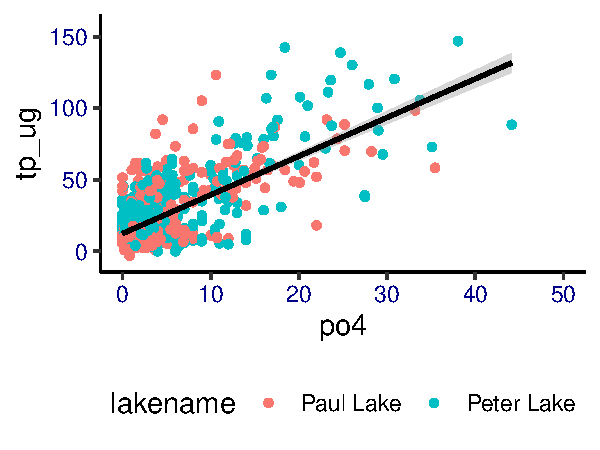
\includegraphics{A05_DataVisualization_files/figure-latex/unnamed-chunk-4-1.pdf}

\begin{enumerate}
\def\labelenumi{\arabic{enumi}.}
\setcounter{enumi}{4}
\tightlist
\item
  {[}NTL-LTER{]} Make three separate boxplots of (a) temperature, (b)
  TP, and (c) TN, with month as the x axis and lake as a color
  aesthetic. Then, create a cowplot that combines the three graphs. Make
  sure that only one legend is present and that graph axes are aligned.
\end{enumerate}

\begin{Shaded}
\begin{Highlighting}[]
\FunctionTok{library}\NormalTok{(cowplot)}
\end{Highlighting}
\end{Shaded}

\begin{verbatim}
## Warning: package 'cowplot' was built under R version 3.6.3
\end{verbatim}

\begin{Shaded}
\begin{Highlighting}[]
\CommentTok{\#5}
\NormalTok{NTL}\SpecialCharTok{$}\NormalTok{month }\OtherTok{\textless{}{-}} \FunctionTok{as.character}\NormalTok{(NTL}\SpecialCharTok{$}\NormalTok{month)}
\CommentTok{\#(a)}
\NormalTok{TEMM }\OtherTok{\textless{}{-}}
  \FunctionTok{ggplot}\NormalTok{(NTL, }\FunctionTok{aes}\NormalTok{(}\AttributeTok{x =}\NormalTok{ month, }\AttributeTok{y =}\NormalTok{ temperature\_C)) }\SpecialCharTok{+}
  \FunctionTok{geom\_boxplot}\NormalTok{(}\FunctionTok{aes}\NormalTok{(}\AttributeTok{color =}\NormalTok{ lakename)) }\SpecialCharTok{+}
  \FunctionTok{theme}\NormalTok{(}\AttributeTok{legend.position =} \StringTok{"none"}\NormalTok{)}
\CommentTok{\#(b)}
\NormalTok{TPM }\OtherTok{\textless{}{-}}
  \FunctionTok{ggplot}\NormalTok{(NTL, }\FunctionTok{aes}\NormalTok{(}\AttributeTok{x =}\NormalTok{ month, }\AttributeTok{y =}\NormalTok{ tp\_ug)) }\SpecialCharTok{+}
  \FunctionTok{geom\_boxplot}\NormalTok{(}\FunctionTok{aes}\NormalTok{(}\AttributeTok{color =}\NormalTok{ lakename)) }\SpecialCharTok{+}
  \FunctionTok{theme}\NormalTok{(}\AttributeTok{legend.position =} \StringTok{"none"}\NormalTok{)}
\CommentTok{\#(c)}
\NormalTok{TNM }\OtherTok{\textless{}{-}}
  \FunctionTok{ggplot}\NormalTok{(NTL, }\FunctionTok{aes}\NormalTok{(}\AttributeTok{x =}\NormalTok{ month, }\AttributeTok{y =}\NormalTok{ tn\_ug)) }\SpecialCharTok{+}
  \FunctionTok{geom\_boxplot}\NormalTok{(}\FunctionTok{aes}\NormalTok{(}\AttributeTok{color =}\NormalTok{ lakename)) }\SpecialCharTok{+}
  \FunctionTok{theme}\NormalTok{(}\AttributeTok{legend.position =} \StringTok{"none"}\NormalTok{)}

\NormalTok{legend\_a }\OtherTok{\textless{}{-}} \FunctionTok{get\_legend}\NormalTok{(TEMM }\SpecialCharTok{+} \FunctionTok{theme}\NormalTok{(}\AttributeTok{legend.position=}\StringTok{"bottom"}\NormalTok{))}
\end{Highlighting}
\end{Shaded}

\begin{verbatim}
## Warning: Removed 3566 rows containing non-finite values (stat_boxplot).
\end{verbatim}

\begin{Shaded}
\begin{Highlighting}[]
\NormalTok{complot }\OtherTok{\textless{}{-}} \FunctionTok{plot\_grid}\NormalTok{(TEMM, TPM, TNM, }\AttributeTok{align =} \StringTok{\textquotesingle{}vh\textquotesingle{}}\NormalTok{, }\AttributeTok{nrow =} \DecValTok{1}\NormalTok{)}
\end{Highlighting}
\end{Shaded}

\begin{verbatim}
## Warning: Removed 3566 rows containing non-finite values (stat_boxplot).
\end{verbatim}

\begin{verbatim}
## Warning: Removed 20729 rows containing non-finite values (stat_boxplot).
\end{verbatim}

\begin{verbatim}
## Warning: Removed 21583 rows containing non-finite values (stat_boxplot).
\end{verbatim}

\begin{Shaded}
\begin{Highlighting}[]
\NormalTok{complot1 }\OtherTok{\textless{}{-}} \FunctionTok{plot\_grid}\NormalTok{(complot, legend\_a , }\AttributeTok{ncol =} \DecValTok{1}\NormalTok{, }\AttributeTok{rel\_heights =} \FunctionTok{c}\NormalTok{(}\DecValTok{3}\NormalTok{,.}\DecValTok{2}\NormalTok{))}
\FunctionTok{print}\NormalTok{(complot1)}
\end{Highlighting}
\end{Shaded}

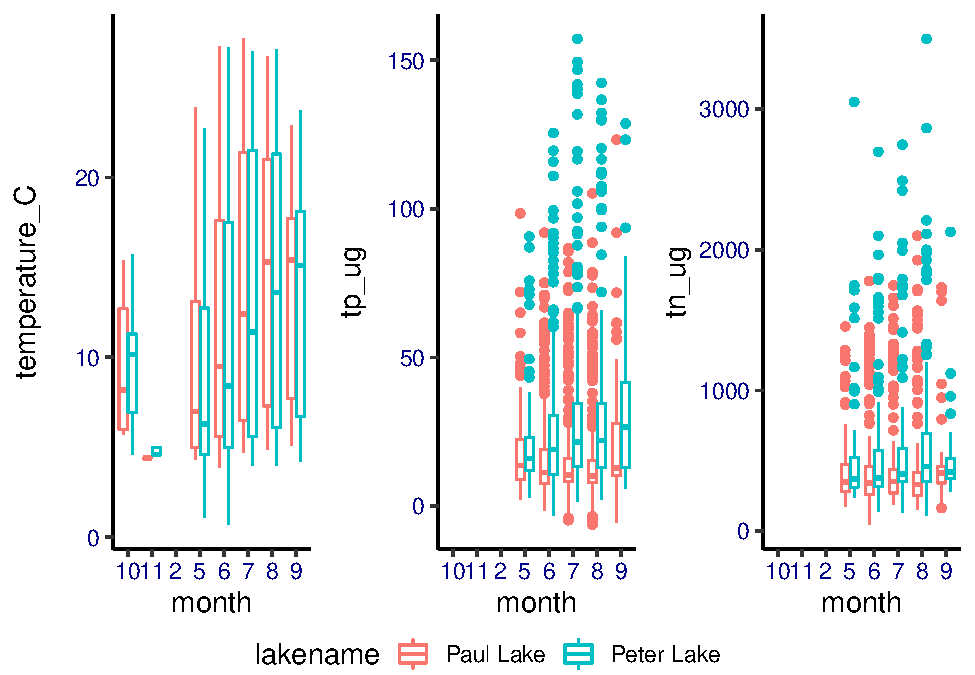
\includegraphics{A05_DataVisualization_files/figure-latex/unnamed-chunk-5-1.pdf}

Question: What do you observe about the variables of interest over
seasons and between lakes? \textgreater{} Answer: \#For temeprature,
lakes have the highest temperature in summer, and lowest temperature in
winter. The temepratures in spring and autumn are mild. The two lakes
have very similar temeprature, but ususally Paul lake has higher average
temeprature than Peter Lake. \#For total phosphorus(tp\_ug), in Peter
Lake, it is higher in summer and lower in spring. BUt, in Paul Lake, it
is consistent; in summer, there is only a slightly lower TP. Peter lake
has higher tp\_ug than Paul lake. \#For total nutrients (tn\_ug), it is
generally consistent for every lake. Peter lake may have a sligtly
higher nutrient level in August. And, Peter lake has higher total
nutrients than Paul Lake.

\begin{enumerate}
\def\labelenumi{\arabic{enumi}.}
\setcounter{enumi}{5}
\item
  {[}Niwot Ridge{]} Plot a subset of the litter dataset by displaying
  only the ``Needles'' functional group. Plot the dry mass of needle
  litter by date and separate by NLCD class with a color aesthetic. (no
  need to adjust the name of each land use)
\item
  {[}Niwot Ridge{]} Now, plot the same plot but with NLCD classes
  separated into three facets rather than separated by color.
\end{enumerate}

\begin{Shaded}
\begin{Highlighting}[]
\CommentTok{\#6}
\NormalTok{Needles1 }\OtherTok{\textless{}{-}} 
  \FunctionTok{ggplot}\NormalTok{(}\FunctionTok{subset}\NormalTok{(NEON, functionalGroup }\SpecialCharTok{==} \StringTok{"Needles"}\NormalTok{), }
         \FunctionTok{aes}\NormalTok{(}\AttributeTok{x =}\NormalTok{ collectDate, }\AttributeTok{y =}\NormalTok{ dryMass, }\AttributeTok{color=}\NormalTok{nlcdClass)) }\SpecialCharTok{+} 
  \FunctionTok{geom\_point}\NormalTok{()}
\FunctionTok{print}\NormalTok{(Needles1)}
\end{Highlighting}
\end{Shaded}

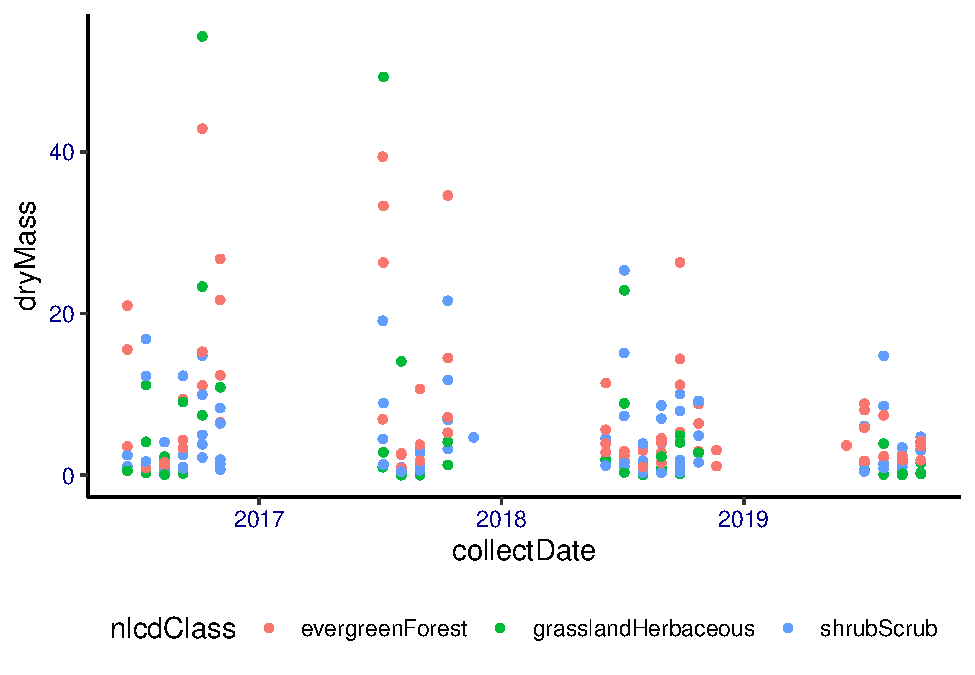
\includegraphics{A05_DataVisualization_files/figure-latex/unnamed-chunk-6-1.pdf}

\begin{Shaded}
\begin{Highlighting}[]
\CommentTok{\#7}
\NormalTok{Needles2 }\OtherTok{\textless{}{-}}
  \FunctionTok{ggplot}\NormalTok{(}\FunctionTok{subset}\NormalTok{(NEON, functionalGroup }\SpecialCharTok{==} \StringTok{"Needles"}\NormalTok{), }
         \FunctionTok{aes}\NormalTok{(}\AttributeTok{x =}\NormalTok{ collectDate, }\AttributeTok{y =}\NormalTok{ dryMass, }\AttributeTok{color=}\NormalTok{nlcdClass)) }\SpecialCharTok{+}
  \FunctionTok{geom\_point}\NormalTok{() }\SpecialCharTok{+}
  \FunctionTok{facet\_wrap}\NormalTok{(}\FunctionTok{vars}\NormalTok{(nlcdClass), }\AttributeTok{nrow =} \DecValTok{1}\NormalTok{)}
\FunctionTok{print}\NormalTok{(Needles2)}
\end{Highlighting}
\end{Shaded}

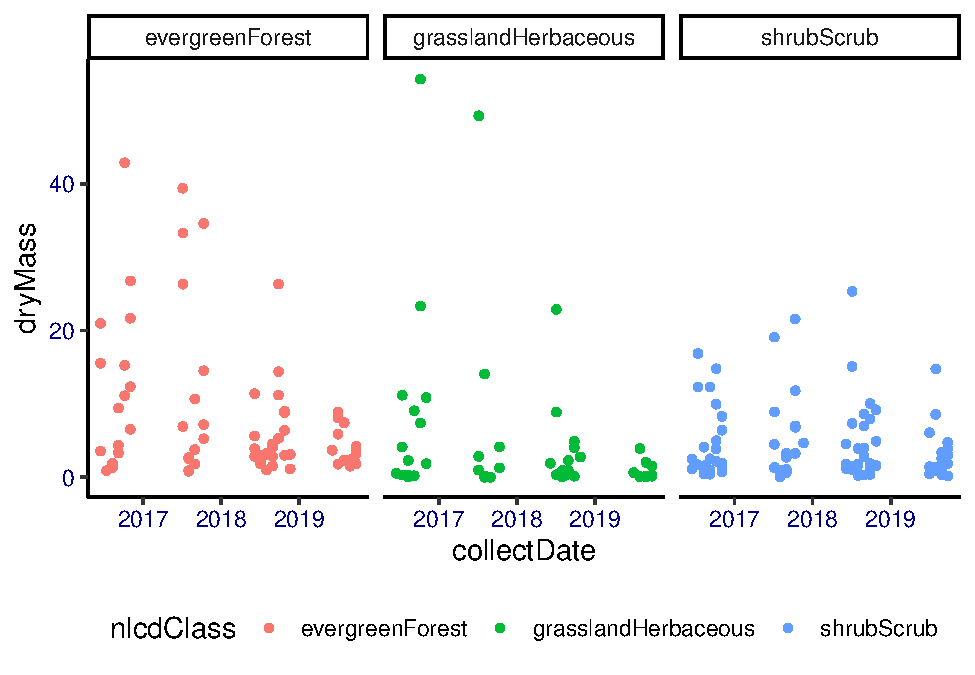
\includegraphics{A05_DataVisualization_files/figure-latex/unnamed-chunk-6-2.pdf}
Question: Which of these plots (6 vs.~7) do you think is more effective,
and why?

\begin{quote}
Answer: I think the plot in \#7 is more effective, because all the dots
in the same class can be clearly observed. However, the plot \#6 many
dots in different classes overlapped with each other, which makes the
trend hard to observe.
\end{quote}


\end{document}
